\documentclass[xcolor=dvipsnames]{beamer}

% ==== 主題 ====
\usetheme{metropolis}
\usefonttheme{professionalfonts}          % 不覆蓋你自訂的字型

% ==== 字型 ====
\usepackage{fontspec}
\usepackage{xeCJK}
\renewcommand{\familydefault}{\rmdefault} % 使用 serif 字體(重點)

% 西文字型:Times New Roman 的開源替代品
\setmainfont{TeX Gyre Termes}[
  Ligatures=TeX,
  BoldFont={* Bold},
  ItalicFont={* Italic}
]

% 中文字型(可改為思源宋體、標楷體等)
\setCJKmainfont{Noto Serif CJK TC}
\setCJKsansfont{Noto Sans CJK TC} % 有需要再用
\setCJKmonofont{Noto Sans Mono CJK TC}

% ==== 數學字型(與正文字體一致)====
\usepackage{unicode-math}
\setmathfont{TeX Gyre Termes Math}

% ==== 套件 ====
\usepackage{amsmath, amssymb}
\usepackage{graphicx}
\usepackage{hyperref}
\usepackage{minted}
\usepackage{fvextra}
\usepackage{xcolor}
\usepackage{booktabs}

% ==== 顏色設定(可選)====
\definecolor{MyBlue}{RGB}{3, 55, 105}
\setbeamercolor{structure}{fg=MyBlue}
\setbeamercolor{block title}{bg=MyBlue,fg=white}
\setbeamercolor{block body}{bg=blue!5}
\setbeamertemplate{section in toc}{%
  \inserttocsectionnumber.~\inserttocsection\par
}

\setminted{
    linenos,                % 行號
    frame=lines,            % 上下框線
    framesep=5pt,           % 程式碼與邊框距離
    numbersep=8pt,          % 行號與程式碼距離
    fontsize=\scriptsize,   % 字體大小
    breaklines,             % 自動換行
    tabsize=4,              % tab 寬度
    rulecolor=\color{black},% 框線顏色
    xleftmargin=1.5em       % 左側縮排
}

\title{Introduction to C++}
\author{Tai, Wei Hsuan}
\date{week 1}

\begin{document}
	\begin{frame}
		\titlepage
	\end{frame}

    \begin{frame}
        \frametitle{Outline}
        \tableofcontents
    \end{frame}

    \section{課程介紹}

    \begin{frame}
        \frametitle{\href{https://drive.google.com/drive/folders/14Tkn-rddw0k1obeOxkWi00S43M0e9wlW?usp=sharing}{課程簡報}}
        \begin{figure}
            \centering
            
\includegraphics[width=0.7\textwidth]{src/qrcode.png}
        \end{figure}
    \end{frame}

    \begin{frame}
        \frametitle{關於我...}
        \begin{itemize}
            \item 戴偉璿(Tai, Wei Hsuan)
            \item 台大醫工大三
            \item 擅長:C++、資料結構與演算法、網際網路概論、網站前後端架設、Linux、機器學習...
            \item 興趣:寫程式、看棒球、打電動
            \item 張學友的粉絲
        \end{itemize}
    \end{frame}

    \begin{frame}
        \frametitle{進度安排}
        \makebox[\linewidth][c]{%
            \begin{tabular}{cl cl}
            \toprule
            日期 & 主題 & 日期 & 主題 \\
            \midrule
            9/12  & 課程簡介、基礎輸入輸出、變數   & 11/28 & 函式 \\
            9/19  & 變數的運算           & 12/5  & 遞迴 \\
            10/17 & 選擇結構與邏輯運算子     & 12/12 & Struct \\
            10/31 & 重複結構                 & 12/19 & Vector \\
            11/7  & 字串處理                 & 12/26 & Stack, Queue \\
            11/21 & 期中考                   & 1/2   & Set, Map, Priority Queue \\
                &                          & 1/9   & 期末考 \\
            \bottomrule
            \end{tabular}
        }
    \end{frame}

    \begin{frame}
        \frametitle{上課方式}
        \begin{itemize}
            \item 觀念講解、範例示範
            \item 大量的練習題
            \item 大量的數學證明(如果有必要)
            \item 期中考與期末考
            \item Zerojudge Code: \texttt{DXg60o}
        \end{itemize}
    \end{frame}

    \begin{frame}
        \frametitle{關於LLM}
        \begin{itemize}
            \item Large Language Model
            \item ChatGPT、Grok、Claude、Gemini
            \item 以討論取代抄答案
            \item \textbf{請不要叫我檢查你用LLM寫的程式碼!}
        \end{itemize}
    \end{frame}

    \section{Why C++?}
    
    \begin{frame}
        \begin{figure}
            \centering
            
\includegraphics[width=1\textwidth]{src/why_not_App.png}
        \end{figure}
    \end{frame}

    % C++ vs Python
    \begin{frame}
        \frametitle{C++ vs Python}
        \begin{itemize}
            \item C++:
            \begin{itemize}
                \item Compiled Language
                \item Static Typing
                \item High Performance
                \item Working Close to Hardware
            \end{itemize}
            \item Python:
            \begin{itemize}
                \item Interpreted Language
                \item Dynamic Typing
                \item Easy to Learn and Use
                \item Rich Libraries and Frameworks
            \end{itemize}
        \end{itemize}
    \end{frame}

    % C++ is everywhere!
    \begin{frame}
        \frametitle{C++ is everywhere!}
        \begin{itemize}
            \item Operating Systems(Windows、macOS、Linux)
            \item Web Browsers(Chrome、Firefox、Edge)
            \item Game Engines(Unreal Engine、Unity)
            \item Parallel Computing(CUDA、OpenCL)
        \end{itemize}
    \end{frame}

    \section{What is C++?}
    
    %Intro to C++
    \begin{frame}
        \frametitle{Introduction to C++}
        \begin{itemize}
            \item First released in Nokia Bell Labs by Bjarne Stroustrup
            \item C with Classes
            \item 1983s, C with Classes $\rightarrow$ C++
            \item Object-Oriented Programming
            \item Directly manipulate hardware resources(memory, CPU)
        \end{itemize}
    \end{frame}

    \begin{frame}
        \frametitle{"Father" of Programming Languages}
        \begin{itemize}
            \item CPython, Numpy, Pandas, Matplotlib, Scikit-learn, TensorFlow, PyTorch
            \item JavaScript V8 Engine, Node.js, Deno
            \item MySQL, PostgreSQL, MongoDB
            \item Even C++ compiler itself!
        \end{itemize}
    \end{frame}

    \begin{frame}
        \frametitle{Simple C++ IDE}
        \begin{itemize}
            \item Windows: \href{https://sourceforge.net/projects/orwelldevcpp/}{Dev-C++}
            \item macOS: \href{https://developer.apple.com/xcode/}{Xcode}
        \end{itemize}
    \end{frame}

    \section{Basic Structure of C++ Program}

    \begin{frame}[fragile]
        \frametitle{\href{https://zh.wikipedia.org/zh-tw/Hello_Worldtext}{Hello World!}}
        \begin{minted}{cpp}
        #include <iostream>
        using namespace std;

        int main() {
            cout << "Hello World!" << '\n';
            return 0;
        }
        \end{minted}
    \end{frame}

    \begin{frame}
        \frametitle{Three Main Parts}
        \begin{itemize}
            \item Header Files
            \item Namespaces
            \item Main Function
        \end{itemize}
    \end{frame}

    \begin{frame}
        \frametitle{Header Files}
        In python, we use \texttt{import} to include libraries.\\
        In C++, we use \texttt{\#include} to include header files.\\
        The most common header file is \texttt{<iostream>}, which is used for input and output operations(io refers to input/output). But if you want to use other advanced features, you may need to include other header files(i.e. \texttt{<vector>}, \texttt{<algorithm>}). Therefore, we often use \texttt{\#include <bits/stdc++.h>} to include most standard libraries in contests(Do not do this in production code!).

    \end{frame}

    \begin{frame}[fragile]
        \frametitle{Namespaces}
        Header file may contain many functions, classes, and variables. To avoid name conflicts, C++ uses namespaces to group related code together.\\
        Here's an example:
        There's a function called \texttt{sort} in the standard library, and you may also define your own function called \texttt{sort}.
        \begin{minted}{cpp}
        #include <bits/stdc++.h>
        using namespace std;

        void sort(int arr[], int n) {/*sort function here*/}

        int main() {
            int a[] = {3, 1, 2};
            sort(a, 3);
        }            
        \end{minted}
        The code above may cause "ambiguous call" error.
    \end{frame}

    \begin{frame}[fragile]
        Therefore, we need to use an another namespace to wrap our own code.
        \begin{minted}{cpp}
        namespace my_sort {
            void sort(int arr[], int n) {/*sort function here*/}
        }
        \end{minted}
        Or a much easier way, do not use the same name as standard library.
    \end{frame}

    \begin{frame}
        \frametitle{Main Function}
        In your code, you may define lots of functions, global variables, and classes. To tell the compiler where to start executing your program, you need to define a \texttt{main} function.\\
        The \texttt{main} function is the entry point of your program. You can call other functions and use global variables inside the \texttt{main} function.\\
        The concept of main function is similar to\\ \texttt{if \_\_name\_\_ == "\_\_main\_\_":} in Python.
    \end{frame}

    \begin{frame}[fragile]
        \frametitle{Look back to Hello World!}
        \begin{minted}{cpp}
        #include <iostream>
        using namespace std;

        int main() {
            cout << "Hello World!" << '\n';
            return 0;
        }
        \end{minted}
        Practice 1: Zerojudge d483.
    \end{frame}

    \section{Standard Output in C++}
    \begin{frame}
        \frametitle{cout}
        After the explanation of main function, we can now understand much part of it. However, what is \texttt{cout}.
        \texttt{cout} is the standard output stream in C++. It is used to print output to the console.\\Its function is similar to \texttt{print()} in Python.\\
        You can output string, integer, float, and other data types using \texttt{cout}.\\
        If you want to print multiple items, you can use the insertion operator \texttt{<<} to chain them together(To memory the direction of \texttt{<<}, think about the flow of data).\\
        If you want to output a pure variable or number, you can just use \texttt{cout<<variable;}, but if you want to output a string, you need to put it in double quotes(\texttt{" "}). More, if you want to output a single character, you need to put it in single quotes(\texttt{' '}).
    \end{frame}

    \begin{frame}[fragile]
        \frametitle{Example of cout}
        Here's an example of using \texttt{cout}:
        \begin{minted}{cpp}
        int main(){
            string name = "World";
            cout<<"Hello"<<name<<"!"<<'\n';
        }
        \end{minted}
        In this case, name is a variable that stores the string "World". What do you think the output will be?
    \end{frame}

    \begin{frame}[fragile]
        \frametitle{Example of cout}
        It will be \texttt{HelloWorld!}. Because there's no space between \texttt{Hello} and \texttt{World!}.\\
        If you want to add a space, you can do it like these:
        \begin{minted}{cpp}
        cout<<"Hello "<<name<<"!"<<'\n';
        cout<<"Hello"<<' '<<name<<"!"<<'\n';
        \end{minted}
        Practice 2: Zerojudge a001.
    \end{frame}

    \begin{frame}
        \frametitle{Escape Characters}
        Sometimes if you want to print a new line, tab, or other special characters (i.e. \texttt{\textbackslash}), you can use escape characters.\\

        \begin{table}[H]
        \begin{tabular}{cc}
        \toprule
        code & Character \\
        \midrule
        \texttt{\textbackslash n} & new line \\
        \texttt{\textbackslash t} & Tab \\
        \texttt{\textbackslash v} & vertical Tab \\
        \texttt{\textbackslash "} & " \\
        \bottomrule
        \end{tabular}
        \end{table}
        TL;DR: If you can't print a special character directly, just add a \texttt{\textbackslash} before it.\\
        Practice 3: Zerojudge e926.
    \end{frame}


    \section{Standard Input \& Variables in C++}
    \begin{frame}[fragile]
        \frametitle{Variables in C++}
        Variables are used to store data in your program.\\
        In Python, you may define a variable like this:
        \begin{minted}{python}
        name = "World"
        age = 18
        \end{minted}
        This is why python is called "weakly typed language".\\
        In C++, you need to specify the data type of the variable when you define it.
        \begin{minted}{cpp}
        string name = "World";
        int age = 18;
        \end{minted}
    \end{frame}

    \begin{frame}
        \frametitle{Data Types in C++}
        Here are some common data types in C++:
        \begin{table}[h]
        \centering
        \caption{Common C++ Fundamental Types}
        \begin{tabular}{cll}
        \toprule
        \textbf{Type} & \textbf{Typical Range} & \textbf{Size (bytes)} \\
        \midrule
        \texttt{int}        & $-2^{31}\sim 2^{31}-1$ & 4 \\
        \texttt{long long}  & $-2^{63}\sim 2^{63}-1$ & 8 \\
        \texttt{float}      & $\pm 1.2 \times 10^{-38}\sim 3.4 \times 10^{38}$ & 4 \\
        \texttt{double}     & $\pm 2.3 \times 10^{-308}\sim 1.7 \times 10^{308}$ & 8 \\
        \texttt{char}       & $-2^7\sim 2^7-1$ & 1 \\
        \texttt{bool}     & 0 or 1 & 1 \\
        \bottomrule
        \end{tabular}
        \end{table}        
    \end{frame}

    \begin{frame}[fragile]
        \frametitle{Input to a Variable}
        You can use \texttt{cin} to get input from the user. For example:
        \begin{minted}{cpp}
        int age;
        cin >>age;
        cout<<"You are "<<age<<" years old."<<'\n';
        \end{minted}
        You can also get multiple inputs in one line:
        \begin{minted}{cpp}
        int dd, mm, yyyy;
        cin >>dd>>mm>>yyyy;
        cout<<"Your birthday is "<<dd<<"/"<<mm<<"/"<<yyyy<<'\n';
        \end{minted}
    \end{frame}

    \begin{frame}
        \frametitle{ASCII}
        In the previous table, you may notice that \texttt{char} stores a number instead of a character.\\
        This is because characters are represented by numbers in the computer. The most common character encoding is ASCII.\\
        For example, the character 'A' is represented by the number 65 in ASCII.\\
        You can use \texttt{int('A')} to get the ASCII value of 'A' in C++.
    \end{frame}

    \begin{frame}
        \begin{figure}
            \centering
            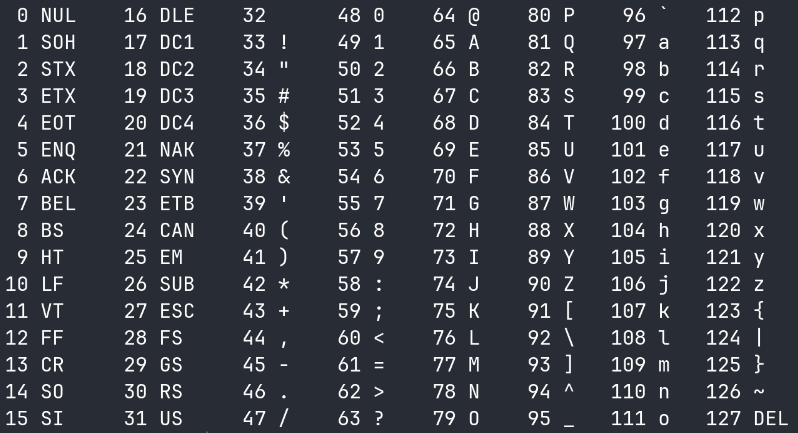
\includegraphics[width=1\textwidth]{src/ASCII.png}
        \end{figure}
    \end{frame}
\end{document}